% TikZ plot for operational metrics
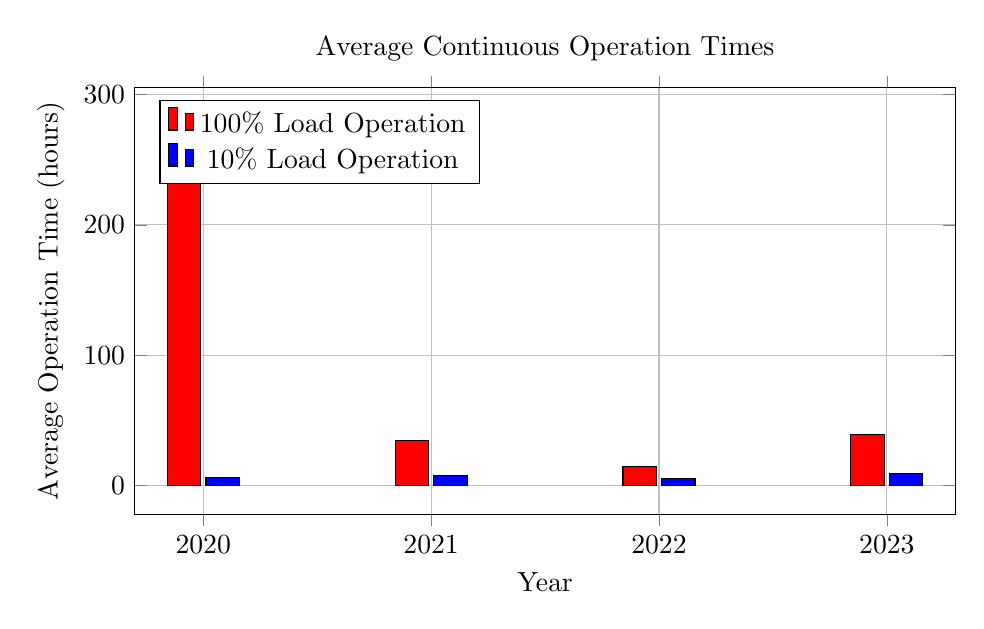
\begin{tikzpicture}
\begin{axis}[
    title={Average Continuous Operation Times},
    xlabel={Year},
    ylabel={Average Operation Time (hours)},
    ybar,
    bar width=12pt,
    width=12cm,
    height=7cm,
    xtick=data,
    xticklabels={2020, 2021, 2022, 2023},
    grid=major,
    legend pos=north west,
]

\addplot[fill=red,draw=black] coordinates {
    (2020, 278.1)
    (2021, 34.7)
    (2022, 14.3)
    (2023, 39.2)
};
\addlegendentry{100\% Load Operation}

\addplot[fill=blue,draw=black] coordinates {
    (2020, 6.3)
    (2021, 7.8)
    (2022, 5.2)
    (2023, 9.4)
};
\addlegendentry{10\% Load Operation}

\end{axis}
\end{tikzpicture}
